\section{Introduction}

\vspace{5 mm}
\noindent
K nearest neighbor is typically applied as a classification method. The 
intuition behind it is given some training data and a new data point, you would 
like to classify the new data based on the class of the training data that it 
is close to. Closeness is defined by a distance metric (e.g. the Euclidean 
distance, absolute distance, some user defined distance metric, etc...) applied 
to the feature space. We find the $k$ closest such data points across the whole 
training data and classify based on a majority class of the $k$ nearest 
training data.

\vspace{5 mm}
\noindent
The K nearest neighbor method of classification works well when similar classes 
are clustered around certain feature spaces [1]. However, the major downside to 
implementing the K nearest neighbor method is it is computationally intense. 
In order to find our new data's $k$ closest observations in the training data, 
we will need to compare its distance to every single training data point. 
If we have training data size $N$, feature space size $P$, and assuming you 
choose a distance metric that is linear in the feature space, we need to 
perform $O(NP)$ computations to determine a single data point's $k$ nearest 
neighbors [2]. This computation will only grow linearly with the amount of new 
observations you wish to predict [3]. With large datasets, this classification 
method becomes prohibitively expensive for traditional serial computing 
paradigms [3].


\vspace{5 mm}
\noindent
K nearest neighbor also has applications beyond direct classification. It can 
be used as a way to approximate the geometric structure of data [2]. It does 
this by finding each data point's $k$ closest data points and ``drawing'' lines 
between them. This is represented by a graph data structure [4], but visually it 
can represent manifolds and geometric structures (see Figure 1).

\begin{figure}[h]
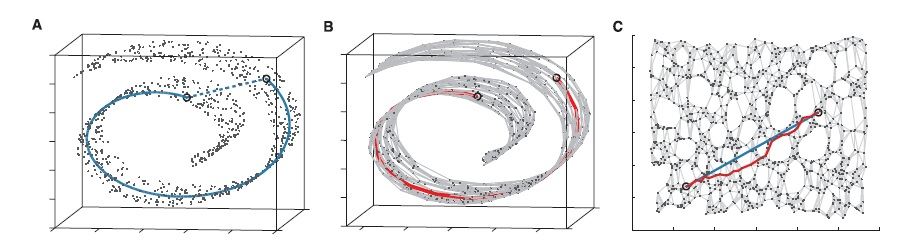
\includegraphics[width=8cm]{manifold}\\
Figure 1: An application of isomaps on a ``swiss roll'' dataset. Notice the 
shape of the date. KNN is used to approximate this shape, then isomaps is used 
to reduce the dimensionality.\\ 
\textit{Source: Lydia E. Kavraki, ``Geometric Methods in Structural
Computational Biology''}
\centering
\end{figure}

\vspace{5 mm}
\noindent
Performing this type of operation is used predominately in manifold learning 
techniques, such as isomaps [4].

\vspace{5 mm}
\noindent
This application of K nearest neighbors is even more computationally heavy 
because now we must compare every point in our data set to every other point. 
Again, a naive implementation would require $O(NP)$ computations per data 
point. However, we would need to do this step $O(N)$ times for each data point, 
thus ultimately requiring $O(N^{2}P)$ computations.
% Not necessary?   \textbf{ADD CITATION}

\vspace{5 mm}
\noindent
We will investigate distributed methods implementing classification with 
K nearest neighbor as well as the geometry of data application. The 
first has a very direct deterministic distributive method. The latter will 
require a randomized approximate approach in order to compute in a distributive 
environment. For the the geometry of data application, we will be mostly 
relaying information learned from \textit{``Clustering Billions of Images with 
Large Scale Nearest Neighbor Search''} [6], where they talk about the use of 
implementing an approximate K nearest neighbor search in a distributed enviornment
using hybrid spill trees.
